\documentclass[10pt, a4paper]{article}
\usepackage{latexsym}
\usepackage{amssymb,amsmath}
\usepackage[pdftex]{graphicx}
\newcommand{\dbar}[1]{\Bar{\Bar{#1}}}

\topmargin = 0.1in \textwidth=5.7in \textheight=8.6in

\oddsidemargin = 0.1in \evensidemargin= 0.1in

% headers
\usepackage{fancyhdr}
\usepackage{bm}
\usepackage{subfigmat}
\usepackage{longtable}
\usepackage{booktabs}
\pagestyle{fancy}
\chead{} 
\rhead{\thepage} 
% footer
\lfoot{\small\scshape } 
\cfoot{} 
%%%% insert your name here %%%%
\rfoot{\footnotesize Burton} 
\renewcommand{\headrulewidth}{.3pt} 
\renewcommand{\footrulewidth}{.3pt}
\setlength\voffset{-0.25in}
\setlength\textheight{648pt}

\begin{document}

\title{Weissinger Vortex Lifting Line as a GP}
\author{Michael Burton}
\maketitle

This write-up describes how the Weissinger Vortex Lifting Line method can be formulated as a signomial program (GP).  

\section*{Weissinger Vortex Lifting Line}

The Weissinger Vortex Lifting Line (WVL) is a lifting line method used to predict aerodynamic forces on a lifting surface.  It uses a collection of horseshoe vortex filaments along the span, each h.v.\ filament having constant strength $\Gamma_i$. 
The equations for the parameters of interest, coefficient of lift $C_L$, and coefficient of induced drag $C_{D_i}$, are 

\begin{align}
    \label{e:cl}
    C_L &= 2 \bar{\Gamma}^{\mathrm{T}} (\bar{V}_x \vec{\Delta y})/S_{\mathrm{ref}} \\
    &= \frac{2}{S_{\mathrm{ref}}} (\bar{\Gamma}_1 \bar{V}_{x_1} \Delta y_1 + \bar{\Gamma}_2 \bar{V}_{x_2} \Delta y_2 + \cdots + \bar{\Gamma}_N \bar{V}_{x_N} \Delta y_N) \nonumber \\
    \label{e:cdi}
    C_{D_i} &= 2 \bar{\Gamma}^{\mathrm{T}} \bar{\bar{B}} \bar{\Gamma}/S_{\mathrm{ref}} \\
            &= \frac{2}{S_{\mathrm{ref}}} (B_{1,1} \Gamma_1^2 + B_{1,2} \Gamma_1 \Gamma_2 + B_{1,3}\Gamma_1 \Gamma_3 + \cdots + B_{N,N} \Gamma_N^2) \nonumber
\end{align}
where the normalized h.v.\ filament strength is $ \bar{\Gamma} = \Gamma/V_{\inf}$, and the local normalized x-component of the velocity is $\bar{V}_x = u/V_{\inf}$.
The h.v.\ filaments can be distributed along the span in a cosine distribution as shown in Figure~\ref{f:wvl}.  

\begin{figure}[h!]
	\begin{center}
	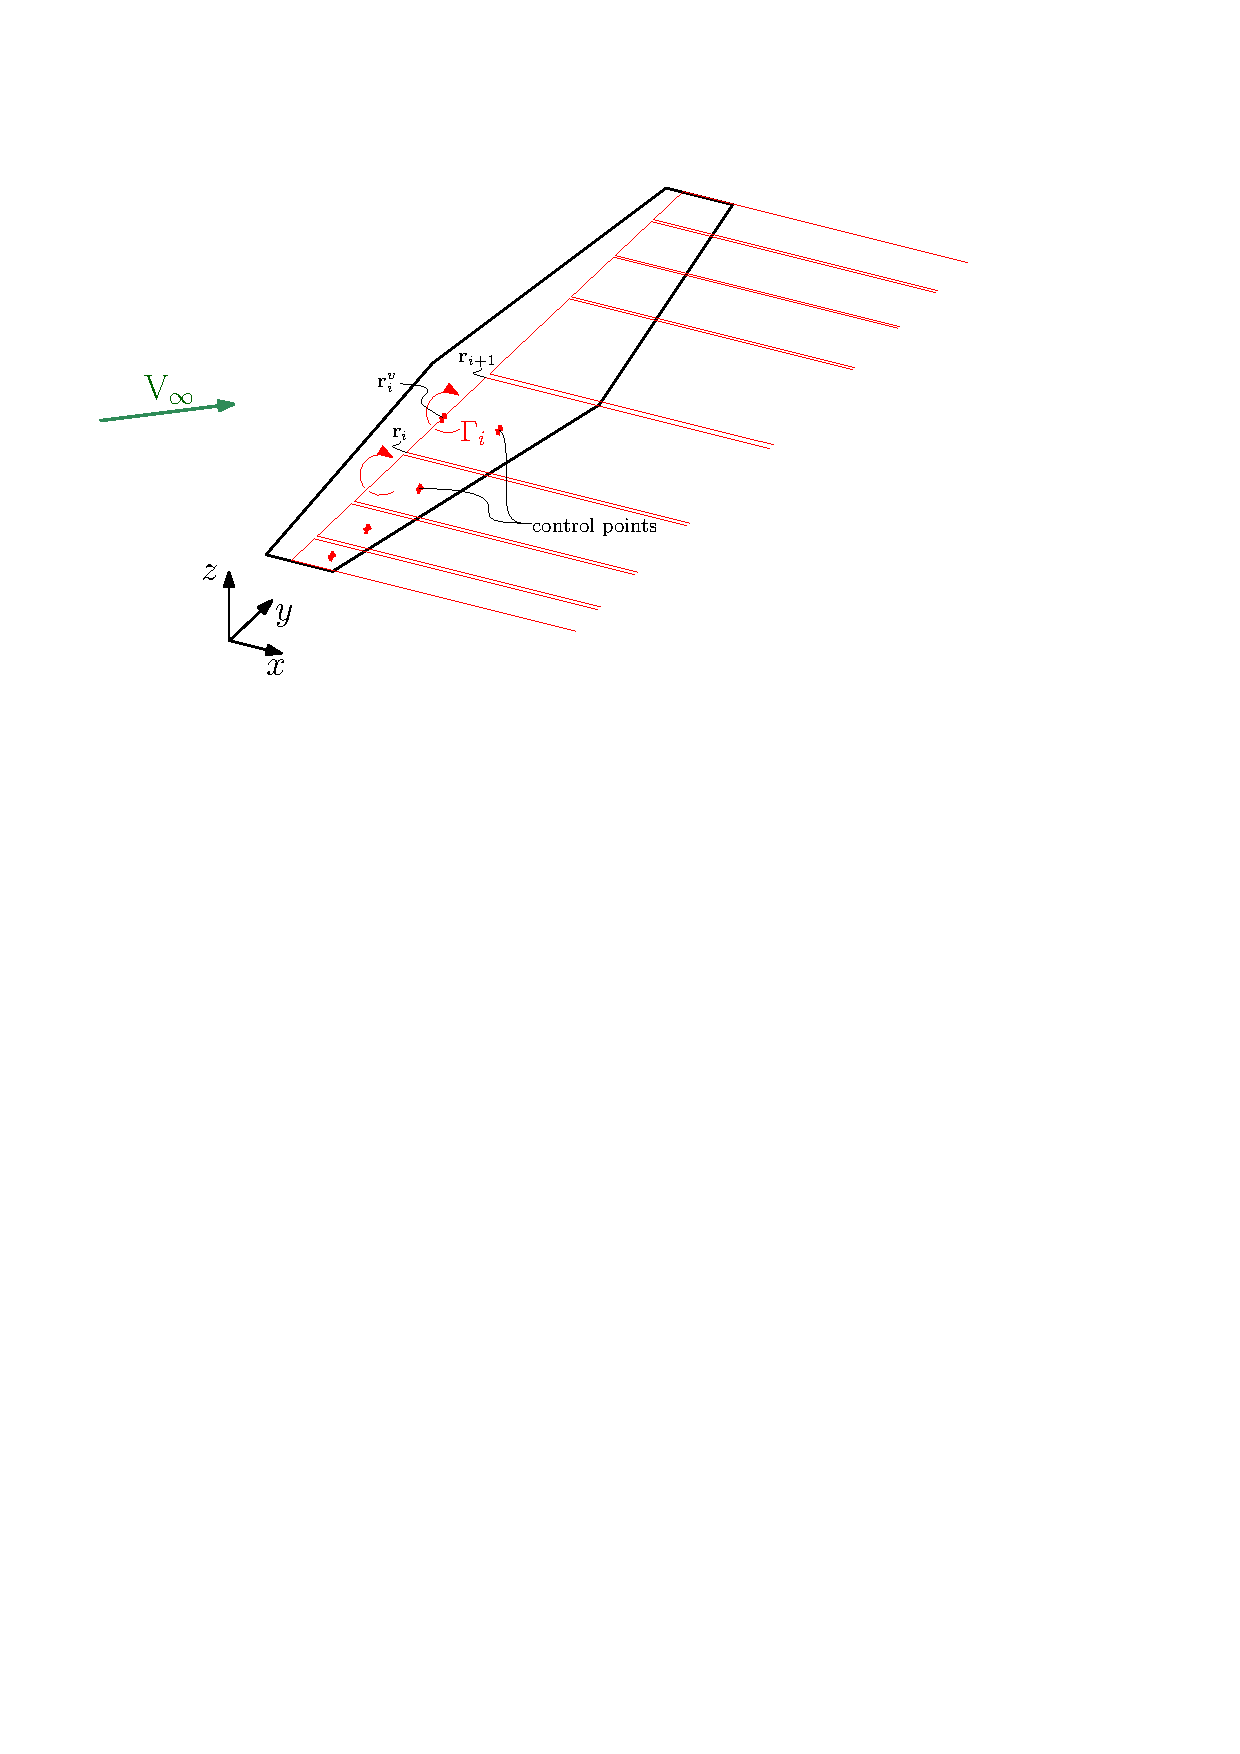
\includegraphics[width=0.8\textwidth]{wvl.pdf}
    \caption{Cosine distribution of h.v.\ filaments on constant taper wing.}
\label{f:wvl}
\end{center}
\end{figure}

The h.v.\ filament strength $\Gamma$, is related to the physical geometry through the Aerodynamic Influence Coefficient (AIC) matrix $\bar{\bar{A}}$, 

\begin{equation}
    \bar{\bar{A}} \bar{\Gamma} = \bar{\mathbf{U}}
\end{equation}
where $\bar{\mathbf{U}}$ is the local normalized velocity vector. The AIC matrix is defined as 

\begin{align}
    A_{ij} &\equiv \hat{\mathbf{V}}_j (\mathbf{r}_i^c) \cdot \bm{n}_{0_i} \\
    \hat{\mathbf{V}}_i (\mathbf{r}) &= \frac{1}{4\pi} \left[ \frac{\mathbf{a} \times \mathbf{b}}{|\mathbf{a}| |\mathbf{b}| + \mathbf{a} \cdot \mathbf{b}} \left( \frac{1}{|\mathbf{a}|} + \frac{1}{|\mathbf{b}|}\right) + \frac{\mathbf{a} \times \hat{\mathbf{x}}}{|\mathbf{a}| - \mathbf{a} \cdot \hat{\mathbf{x}}} \frac{1}{|\mathbf{a}|} - \frac{\mathbf{b} \times \hat{\mathbf{x}}}{|\mathbf{b}| - \mathbf{b} \cdot \hat{\mathbf{x}}} \frac{1}{|\mathbf{b}|} \right]
\end{align}

where the vectors $\bm{\mathrm{a}}$, $\bm{\mathrm{b}}$, and $\bm{\mathrm{x}}$ are defined in Figure~\ref{f:singlehv}. The control vector $\bm{\mathrm{r}}_i^c$ is defined in Figure~\ref{f:singlecp}. 
The WVL method assumes the control vector $\bm{\mathrm{r}}_i^c$ to be a vector to the three-quarters chord $\frac{3}{4}c$.  
The unit normal vector $\bm{n}_{0_i}$, can be approximated as a function of the local twist

\begin{equation}
    \bm{n}_{0_i} \approx \sin{\theta_i} \hat{x} + \cos{\theta_i} \hat{z}
\end{equation}

\begin{figure}[h!]
 \begin{subfigmatrix}{2}% number of columns
\subfigure[$\bm{\mathrm{a}}$, $\bm{\mathrm{b}}$, and $\bm{\mathrm{x}}$ vector definition\label{f:singlehv}]{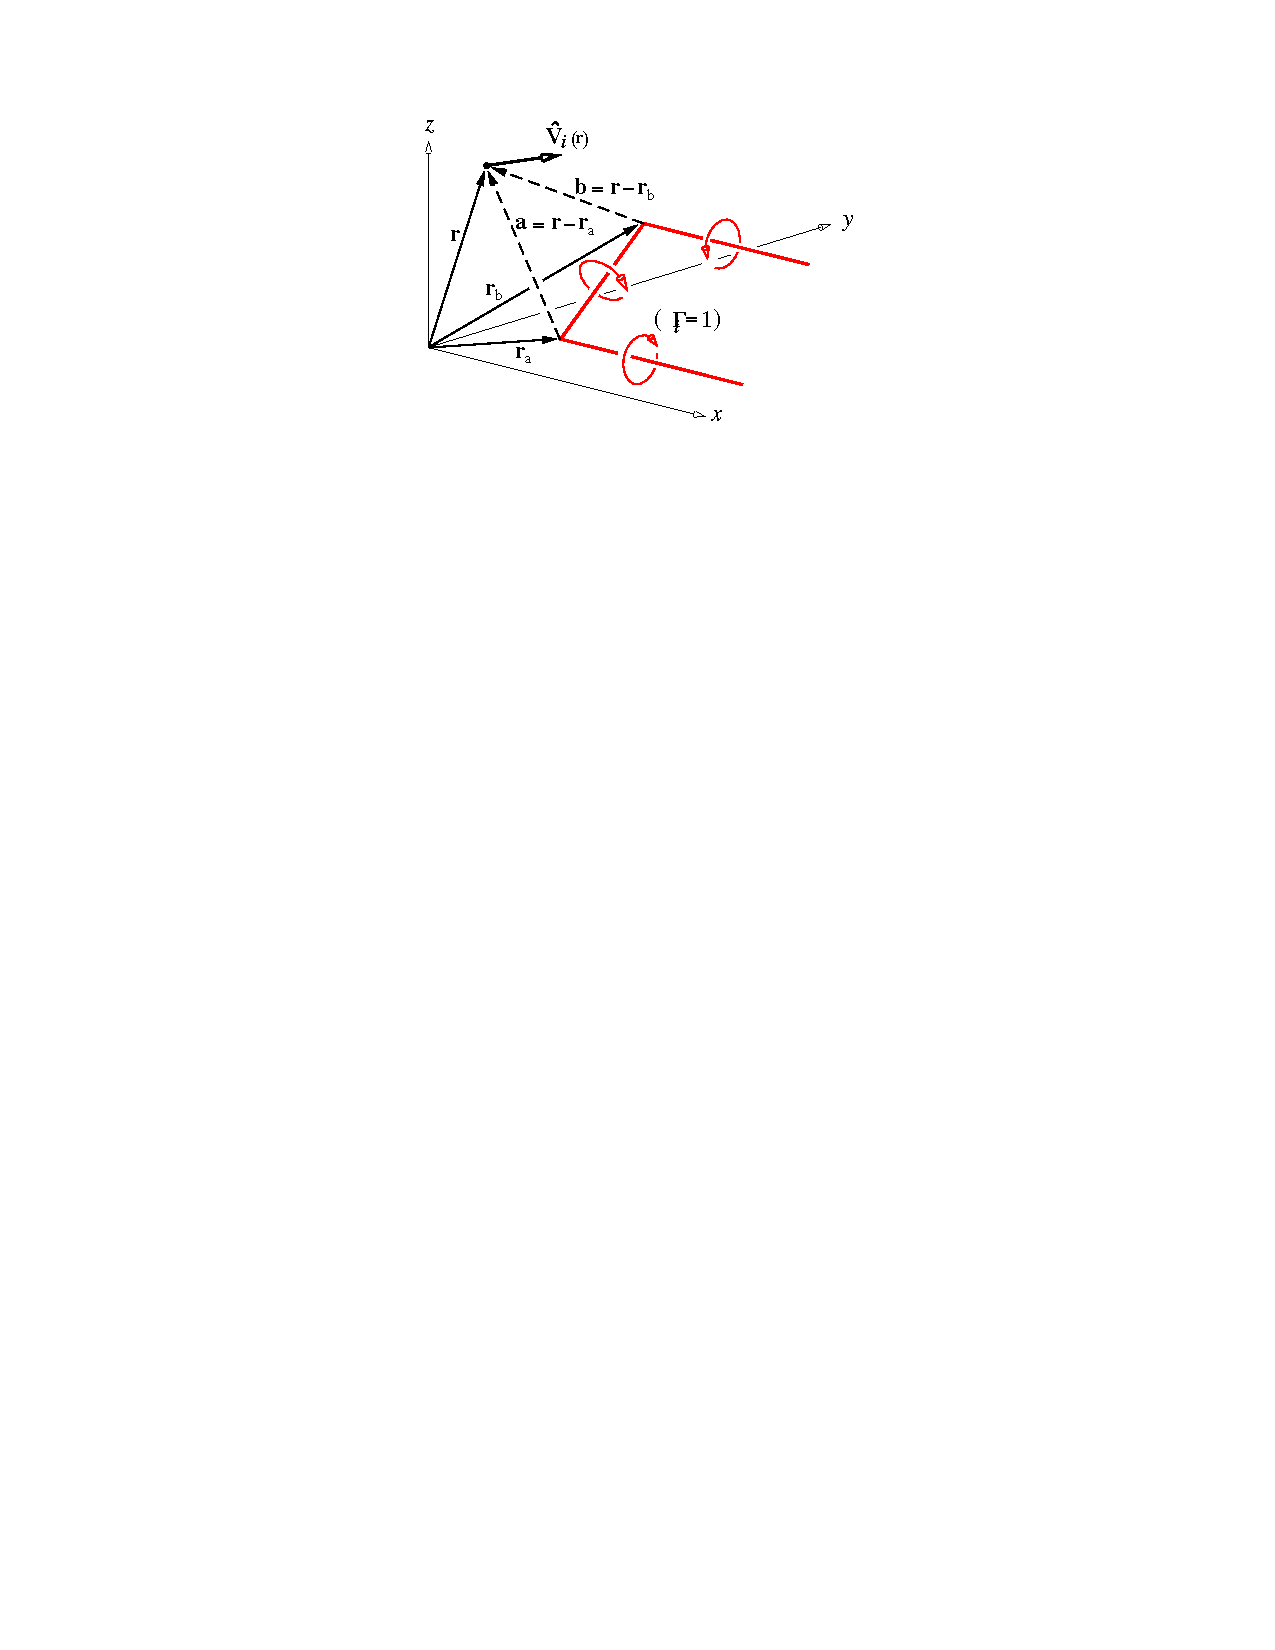
\includegraphics{singlehv.pdf}}
\subfigure[Control vector $\bm{\mathrm{r}}_i^c$ definition\label{f:singlecp}]{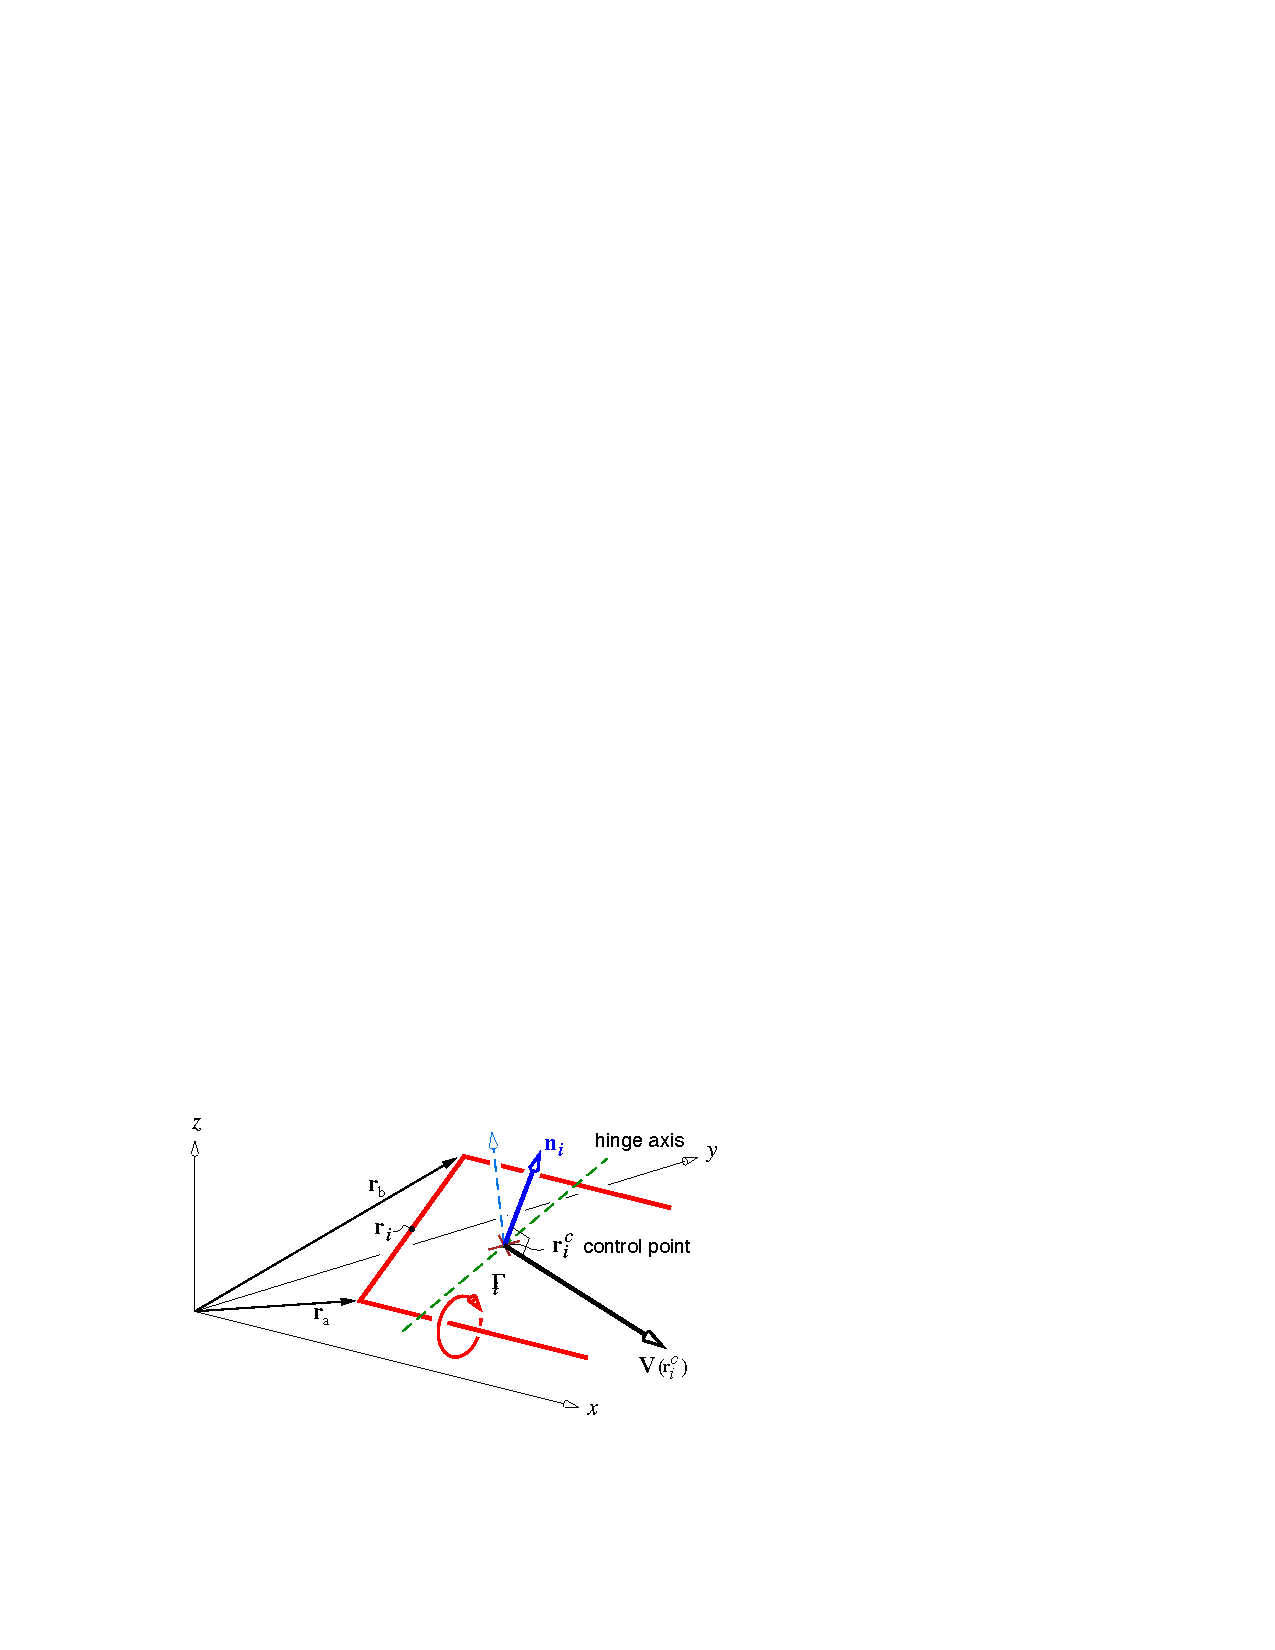
\includegraphics{singlecp.pdf}}
 \end{subfigmatrix}
 \caption{Geometry of one horseshoe vortex.}
\label{f:singlevortex}
\end{figure}

The $\bar{\bar{B}}$ matrix, also a function of the geometry, depends on the vortex midpoint $\mathbf{r}_i^v$, not the control point $\mathbf{r}_i^c$

\begin{align}
    B_{ij} &= \frac{\Delta y_i}{4\pi} \left[ \frac{y_i^v - y_i}{{(y_i^v - y_i)}^2 + {(z_i^v - z_i)}^2} - \frac{y_i^v - y_{i+1}}{{(y_i^v - y_{i+1})}^2 + {(z_i^v - z_{i+1})}^2} \right] \\
    &+ \frac{\Delta z_i}{4\pi} \left[ \frac{z_i^v - y_i}{{(z_i^v - y_i)}^2 + {(z_i^v - z_i)}^2} - \frac{z_i^v - z_{i+1}}{{(y_i^v - y_{i+1})}^2 + {(z_i^v - z_{i+1})}^2} \right] \nonumber
\end{align}

The system of equations can be solved using a Newton method and by specifying flow conditions such as a specified lift coefficient $C_{L_{\mathrm{spec}}}$.

\section*{WVL as a SP:\ Problem Set Up}

A few assumptions are necessary to make the formulation of the Weissenger Lifting Line method compatible as an SP.  It is assumed that the non-dimensional geometric planform definition of the wing is known.  
Specifically, all control vectors $\mathbf{r}_i^c$, node vectors $\mathbf{r}_i$, and midpoint vectors $\mathbf{r}_i^v$ are known.  Thus the AIC matrix $\bar{\bar{A}}$, and the $\bar{\bar{B}}$ matrix are also known.  
Furthermore, it is assumed that that $V_{x_i} = V_{\infty}$.  
Finally, the lift coefficient $C_L$, will be constrained by a specified number $C_{L_{\mathrm{spec}}}$, and the drag coefficient $C_{D_i}$, will be minimized.

These assupmtions allow simplification of Equations~\ref{e:cl} and~\ref{e:cdi} to their SP formulation

\begin{align}
    \text{minimize} & \quad C_{D_i} \nonumber \\
    \label{e:cleq}
    C_{L_{\mathrm{spec}}} &\leq 2 \bar{\Gamma}^{\mathrm{T}} (\vec{\Delta y})/S_{\mathrm{ref}} \\
    \label{e:cdeq}
    C_{D_i} &\geq 2 \bar{\Gamma}^{\mathrm{T}} \bar{\bar{B}} \bar{\Gamma}/S_{\mathrm{ref}}.
\end{align}

\subsection*{Example}

An example case of constant taper wing described in Figure~\ref{f:samplewing} was solved as an SP for a $C_{L_{\mathrm{spec}}} = 1.1$.
The lifting distribution and induced drag were evaluated using a Newton method implementation of the WVL. This solution was compared to the SP solution using 6 h.v.\ filaments. 

\begin{figure}[h!]
	\begin{center}
	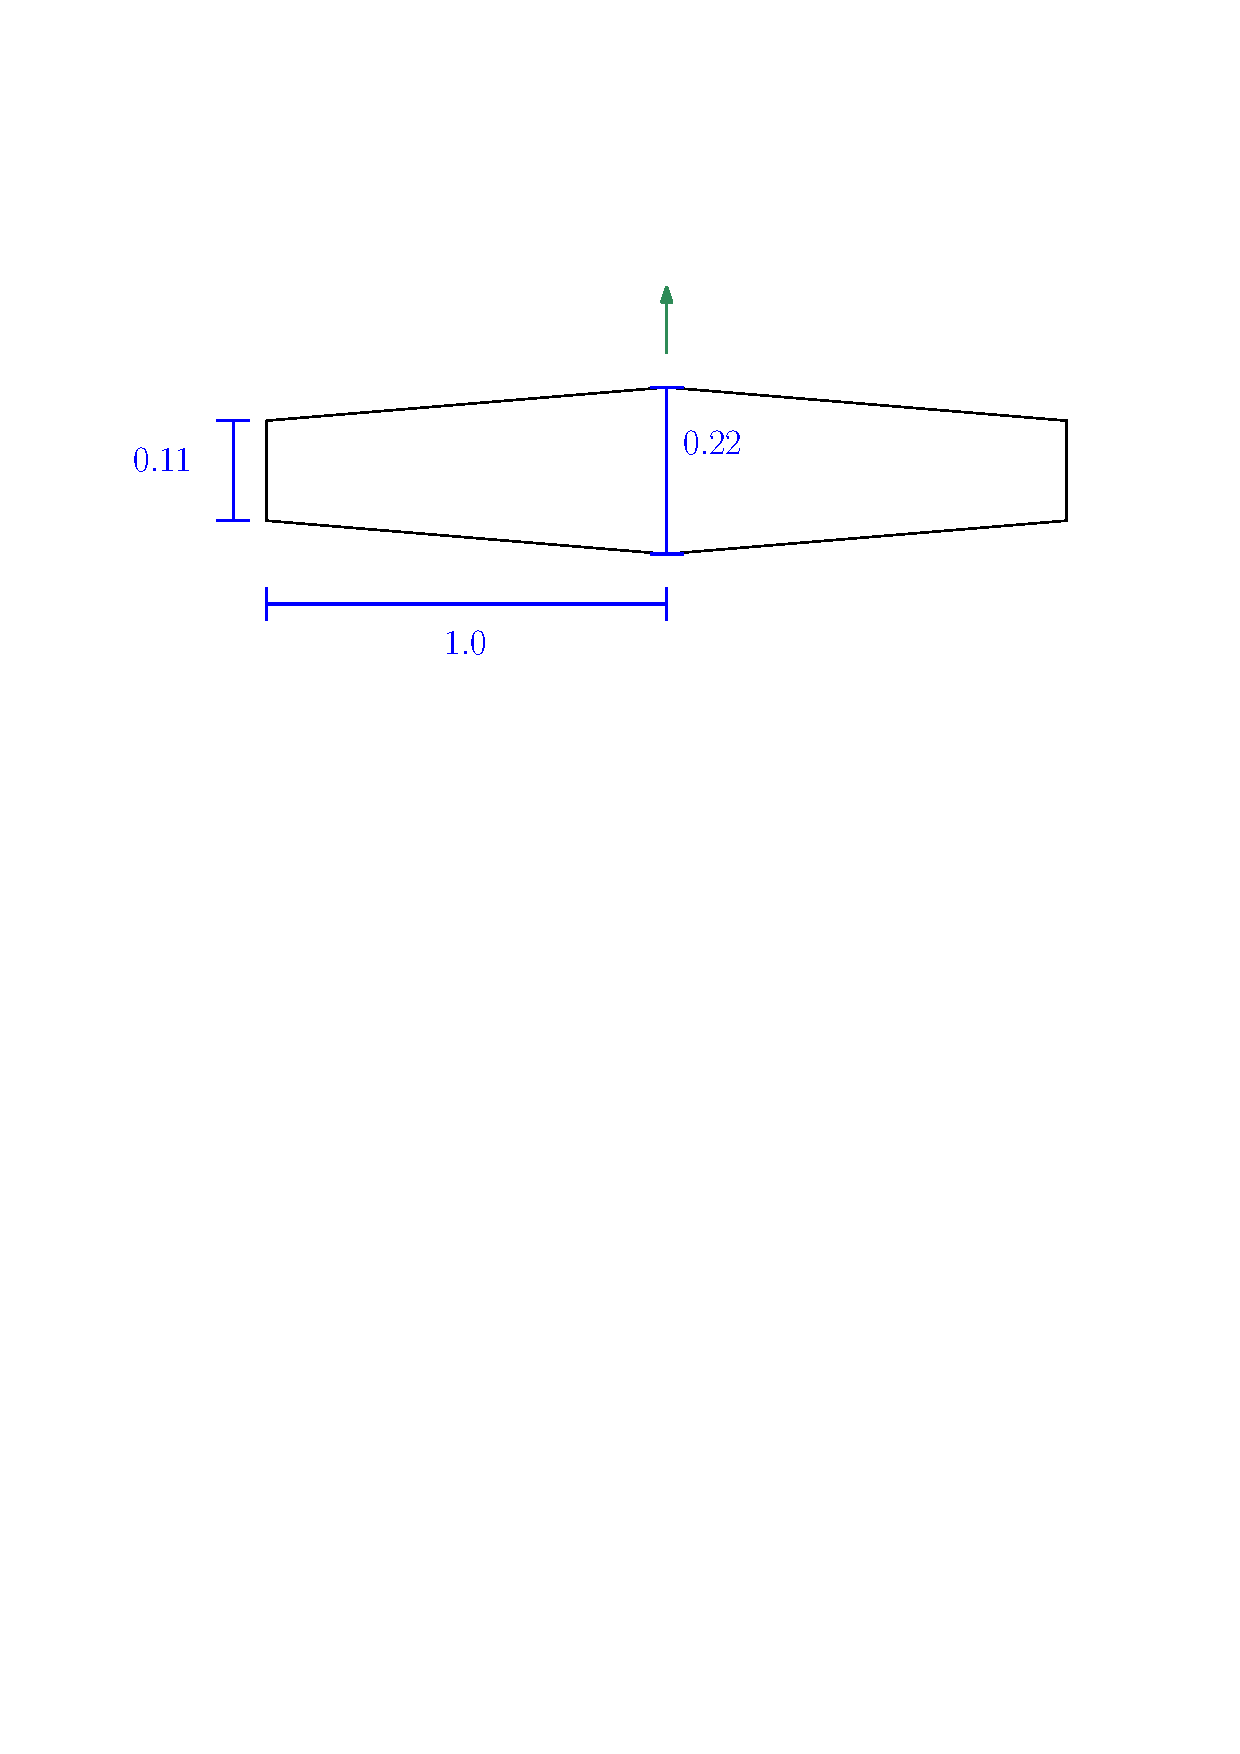
\includegraphics[width=0.8\textwidth]{samplewing.pdf}
    \caption{Sample wing used for comparison between SP model and numerical solution using a Newton method.}
\label{f:samplewing}
\end{center}
\end{figure}

The comparison between $\Gamma$ and $C_{D_i}$ is shown in Table~\ref{t:spcomp}.
Only the first three $\Gamma$ values are shown because the steady level flight condition means the three h.v.\ filaments on the other side of the wing have the same value.  

\begin{longtable}{lccc}
\caption{WVL Method Comparison}\\
\toprule
\toprule
\label{t:spcomp}
Variable            & Newton Method     & SP Model  & Error  \\ \midrule
$C_{D_i} \quad (N=6)$& 0.027             & 0.0263    & 3.0\%  \\
$\bar{\Gamma}_1$    & 0.0565            & 0.0432    & 23\%   \\
$\bar{\Gamma}_2$    & 0.0824            & 0.0850    & 3.2\%  \\
$\bar{\Gamma}_3$    & 0.1070            & 0.1086    & 1.5\%  \\
$C_{D_i} \quad (N=20)$& 0.0307            & 0.0302    & 1.8\%  \\
\bottomrule
\end{longtable}

This comparison shows that the SP model captures the correct trends but is not as accurate as the Newton method.  The SP model solved in 0.15 seconds and took 7 GP solves.  Increasing the number of h.v. filaments to 20 decreases the error, but is still not as accurate.  With $N=20$, the SP model solved in 0.885 seconds and took 15 GP solves. 
 
\end{document}
